\epigraph{``Curious that we spend more time congratulating people who have succeeded than encouraging people who have not."}{Neil deGrasse Tyson}

\section{Open Source Software}
\begin{definition}
Open Source Software is software with source code that anyone can inspect, modify, and enhance. 
\end{definition}

Source code is the code that computer programmers use to modify, and change how a piece of software functions\cite{what_oss}. Programmers with access to the source code can improve that program by adding features to it, fixing bugs, or by improving the documentation of the surrounding source code. 

According to Tom Macaulay\cite{advantages}, the open source development of software has a number of advantages over the traditional development of proprietary software, including but not limited to:

\begin{itemize}
    \item Lower costs.
    \item Extensive customisation.
    \item Higher quality software.
    \item Greater security.
    \item Regular updates.
    \item Quick fixes.
\end{itemize}

If the source code of the software was available to the open source community, it could lead to a low cost, and high quality numerical weather prediction scheme being produced. If such an event occurs, it could, theoretically, vastly enhance existing weather predicting software, and could lead to a further dramatic decline in deaths from weather related phenomena. This project is an attempt to kick start such a future.

Everything related to this project, from the source code of the simulator to this very paper, can be accessed at the organisation known as `AMSIMP' on the open source platform known as GitHub. This can be accessed at \url{https://github.com/amsimp}. 

\begin{figure}[H]
    \centering
    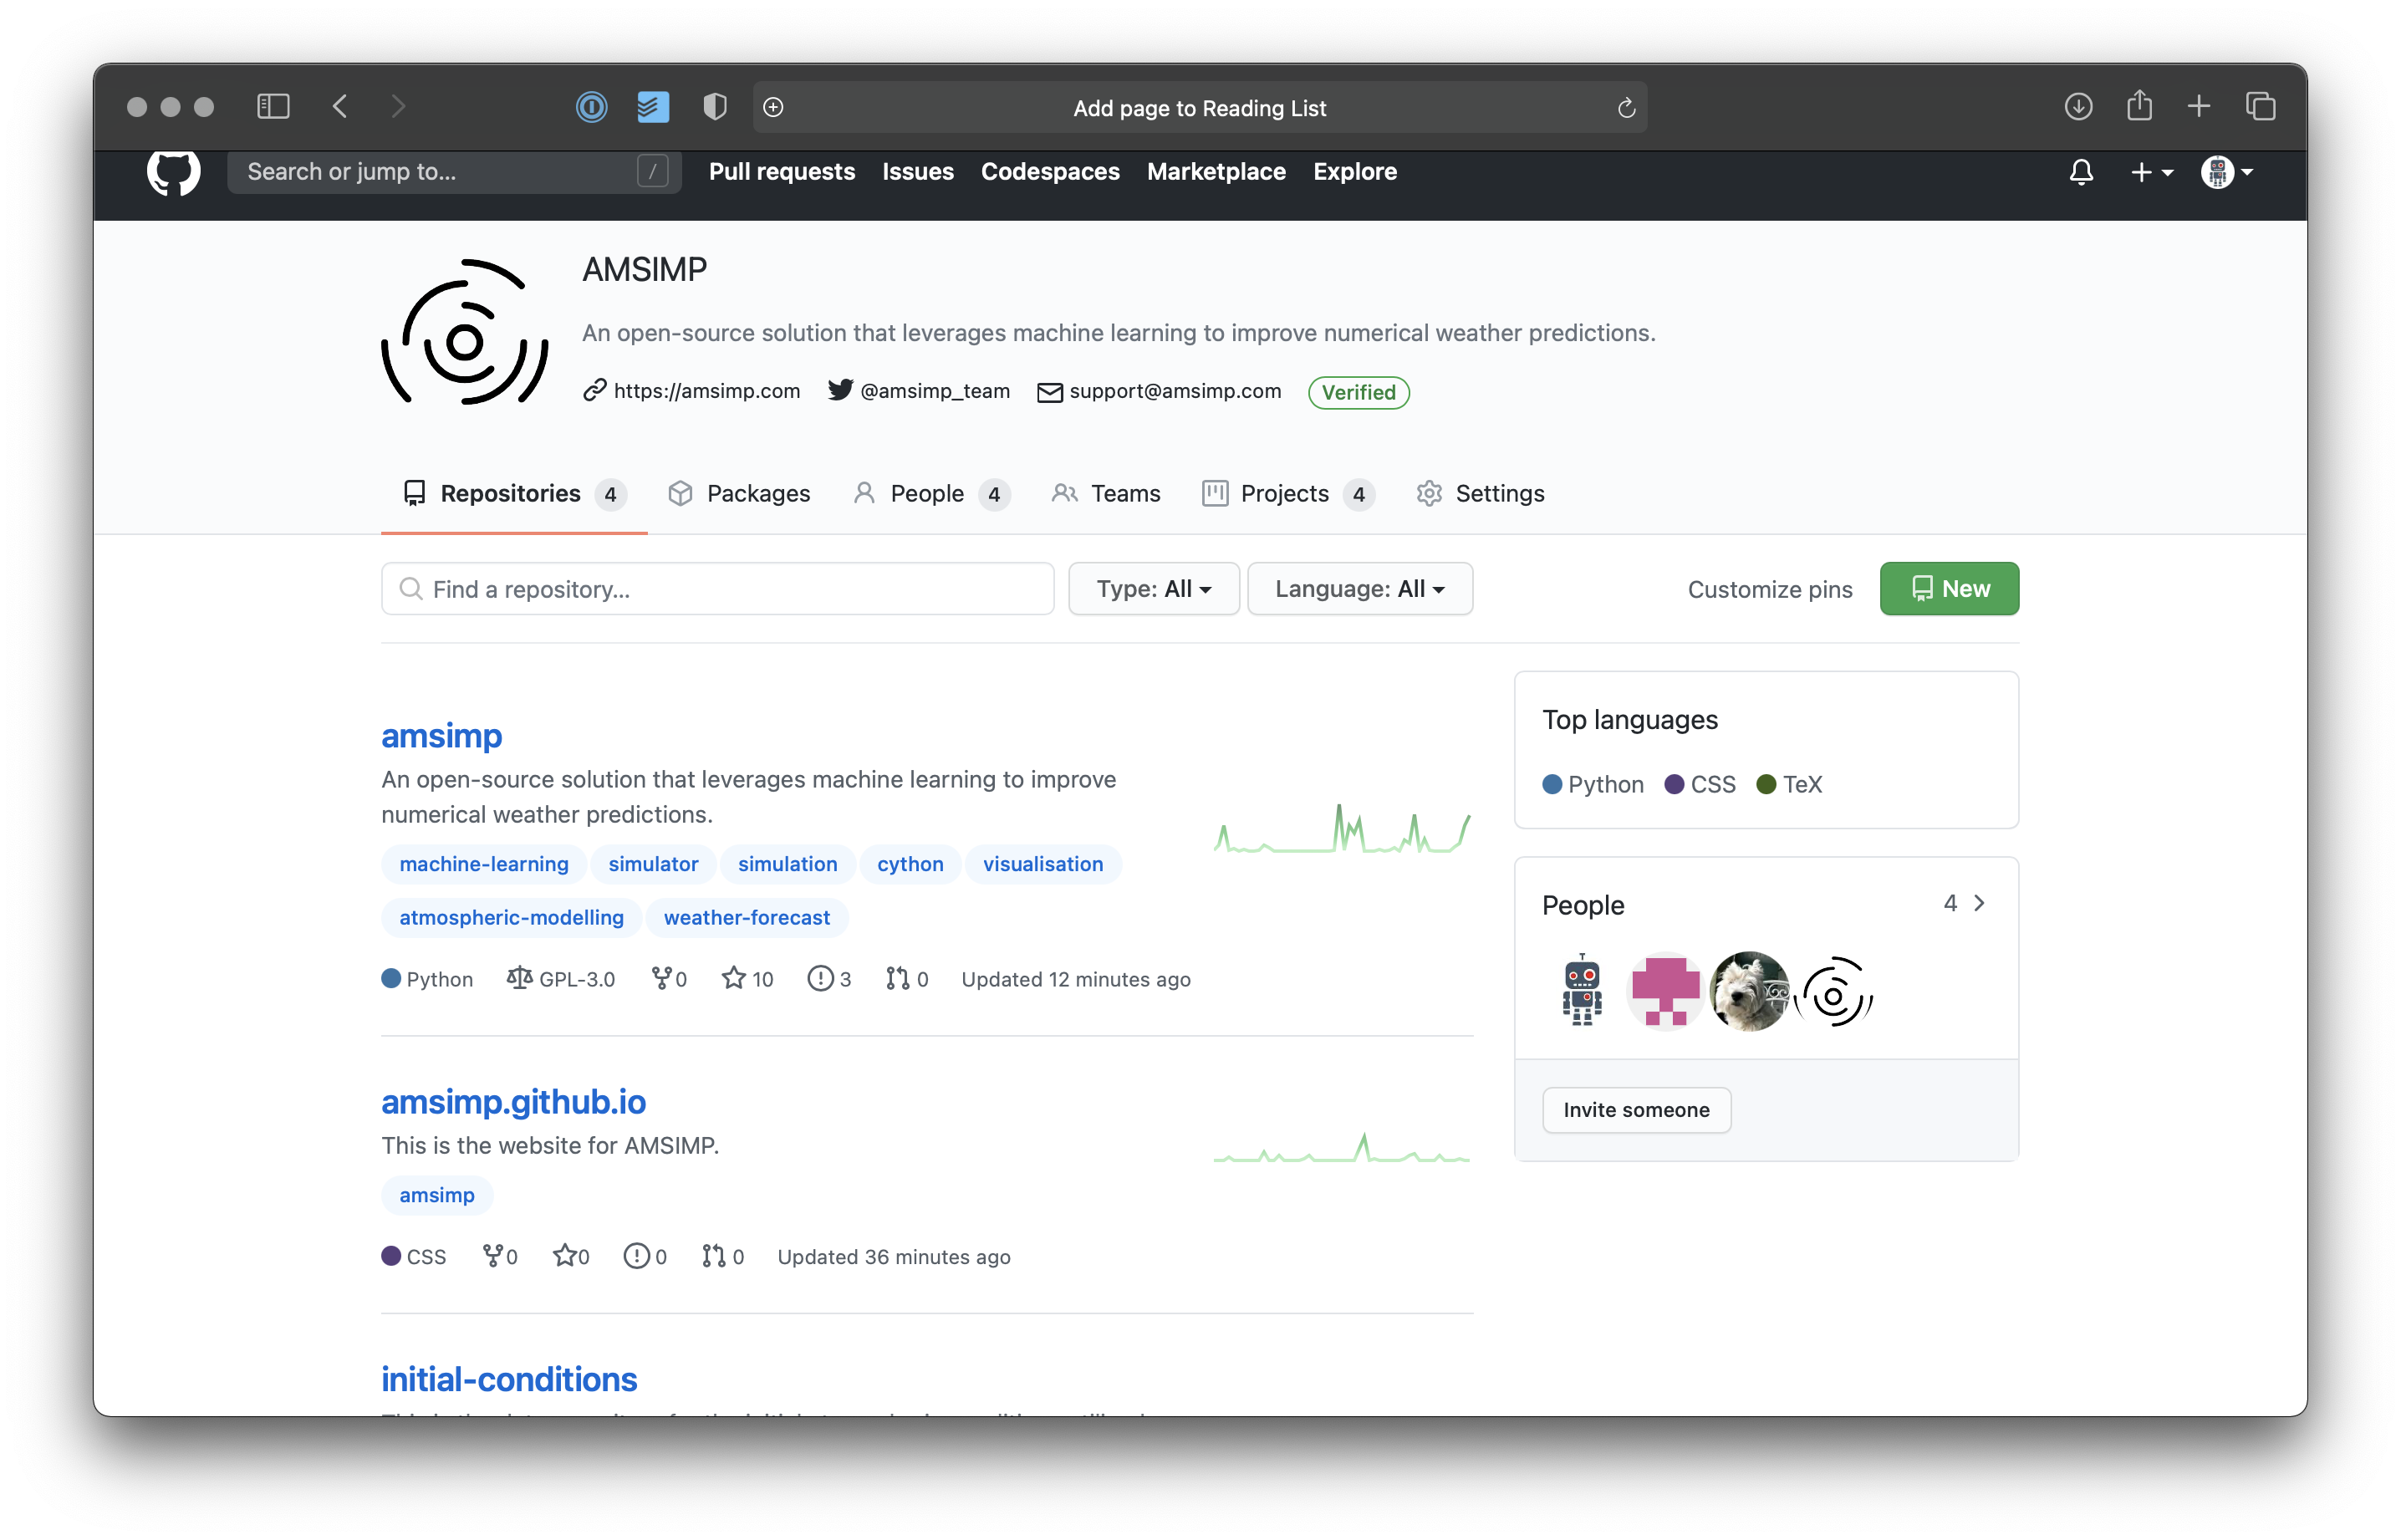
\includegraphics[width=.8\linewidth]{Images/github}
    \caption{A screenshot of the AMSIMP organisation, hosted by the open source platform known as GitHub.}
    \label{github}
\end{figure}

\section{Language Selection}
\subsection{Initial Language Selection}
The most crucial element of this project was choosing an appropriate programming language for the task. During the initial consideration period, I analysed two different programming languages: JavaScript, and Python\cite{python}. 

Initially, I considered the programming language, JavaScript with a run-time environment known as Node.js (Node.js executes code outside of a browser), for two reasons primarily:

\begin{itemize}
    \item JavaScript excels at data visualisation.
    \item Node.js is extremely well suited for memory intensive activities.
\end{itemize}

In line with the expectation of using this programming language, Miss Abbott, and I attended a Dublin Node.js Meetup. I did this in order to gain an understanding of what Node.js is used for, and what would be the best way one would go about using it. 

In the end, however, I ultimately chose Python for the task due to a number of shortcomings on the part of JavaScript (Node.js), and advantages on the part of Python. Firstly, JavaScript just doesn’t have the same enormous suite of scientific packages and inbuilt functionality that Python does. Using JavaScript, therefore, would waste valuable development time, and ultimately would be entirely inefficient.

Secondly, Python already has an extensive ecosystem with how-to’s available for almost any scientific task you would ever want to do. For JavaScript, this is simply not the case.\cite{javascript_vs_python}

